\documentclass[10pt,DIV16,a4paper,abstract=true,twoside=semi,openright]
{scrreprt}
%%%%%%%%%%%%%%%%%%%%%%%%%%%%%%%%%%%%%%%%%%%%%%%%%%%%%%%%%%%%%%%%%%%%%%%
%%% Overrides the (rightfully issued) warnings by Koma Script that \rm
%%% etc. should not be used (they are deprecated since more than a
%%% decade)
  \DeclareOldFontCommand{\rm}{\normalfont\rmfamily}{\mathrm}
  \DeclareOldFontCommand{\sf}{\normalfont\sffamily}{\mathsf}
  \DeclareOldFontCommand{\tt}{\normalfont\ttfamily}{\mathtt}
  \DeclareOldFontCommand{\bf}{\normalfont\bfseries}{\mathbf}
  \DeclareOldFontCommand{\it}{\normalfont\itshape}{\mathit}
%%%%%%%%%%%%%%%%%%%%%%%%%%%%%%%%%%%%%%%%%%%%%%%%%%%%%%%%%%%%%%%%%%%%%%%
\usepackage[english]{babel}
\usepackage[numbers, sort&compress]{natbib}
\usepackage{isabelle,isabellesym}
\usepackage{booktabs}
\usepackage{paralist}
\usepackage{graphicx}
\usepackage{amssymb}
\usepackage{xspace}
\usepackage{xcolor}
\usepackage{listings}
\lstloadlanguages{HTML}
\usepackage[]{mathtools}
\usepackage[pdfpagelabels, pageanchor=false, plainpages=false]{hyperref}
\lstdefinestyle{html}{language=XML,
  basicstyle=\ttfamily,
  commentstyle=\itshape,
  keywordstyle=\color{blue},
  ndkeywordstyle=\color{blue},
}
\lstdefinestyle{displayhtml}{style=html,
  floatplacement={tbp},
  captionpos=b,
  framexleftmargin=0pt,
  basicstyle=\ttfamily\scriptsize,
  backgroundcolor=\color{black!2},
  frame=lines,
}
\lstnewenvironment{html}[1][]{\lstset{style=displayhtml, #1}}{}
\def\inlinehtml{\lstinline[style=html, columns=fullflexible]}

\pagestyle{headings}
\isabellestyle{default}
\setcounter{tocdepth}{1}
\newcommand{\ie}{i.\,e.\xspace}
\newcommand{\eg}{e.\,g.\xspace}
\newcommand{\thy}{\isabellecontext}
\renewcommand{\isamarkupsection}[1]{%
  \begingroup% 
  \def\isacharunderscore{\textunderscore}%
  \section{#1 (\thy)}%
  \endgroup% 
}

\title{Core DOM\\\medskip \Large 
  A Formal Model of the Document Object Model}%
\author{Achim~D.~Brucker \and Michael~Herzberg}%
\publishers{
  Department of Computer Science\\
  The University of Sheffield\\
  Sheffield, UK\\
  \texttt{\{\href{mailto:a.brucker@sheffield.ac.uk}{a.brucker},
    \href{mailto:msherzberg1@sheffield.ac.uk}{msherzberg1}\}@sheffield.ac.uk}
}
\begin{document}
  \maketitle
  \begin{abstract}
    \begin{quote}
    In this AFP entry, we formalize the core of the Document Object
    Model (DOM).  At its core, the DOM defines a tree-like data
    structure for representing documents in general and HTML documents
    in particular. It is the heart of any modern web browser.

    Formalizing the key concepts of the DOM is a prerequisite for the
    formal reasoning over client-side JavaScript programs and for the
    analysis of security concepts in modern web browsers.

    
    We present a formalization of the core DOM, with focus on the
    \emph{node-tree} and the operations defined on node-trees, in
    Isabelle/HOL\@. We use the formalization to verify the functional
    correctness of the most important functions defined in the DOM
    standard. Moreover, our formalization is
    \begin{inparaenum}
    \item \emph{extensible}, i.e., can be extended without the need of
      re-proving already proven properties and
    \item \emph{executable}, i.e., we can generate executable code
      from our specification.
    \end{inparaenum}

    \bigskip
    \noindent{\textbf{Keywords:}} 
      Document Object Model, DOM, Formal Semantics, Isabelle/HOL      
    \end{quote}
  \end{abstract}


\tableofcontents
\cleardoublepage

\chapter{Introduction}
In a world in which more and more applications are offered as services
on the internet, web browsers start to take on a similarly central
role in our daily IT infrastructure as operating systems. Thus, web
browsers should be developed as rigidly and formally as operating
systems. While formal methods are a well-established technique in the
development of operating systems (see,
\eg,~\citet{klein:operating:2009} for an overview of formal
verification of operating systems), there are few proposals for
improving the development of web browsers using formal
approaches~\cite{gardner.ea:dom:2008,raad.ea:dom:2016,jang.ea:establishing:2012,bohannon.ea:featherweight:2010}.

As a first step towards a verified client-side web application stack,
we model and formally verify the Document Object Model (DOM) in
Isabelle/HOL\@. The DOM~\cite{whatwg:dom:2017,w3c:dom:2015} is
\emph{the} central data structure of all modern web browsers.  At its
core, the Document Object Model (DOM), defines a tree-like data
structure for representing documents in general and HTML documents in
particular. Thus, the correctness of a DOM implementation is crucial
for ensuring that a web browser displays web pages correctly.
Moreover, the DOM is the core data structure underlying client-side
JavaScript programs, \ie, client-side JavaScript programs are mostly
programs that read, write, and update the DOM.

In more detail, we formalize the core DOM as a shallow
embedding~\cite{joyce.ea:higher:1994} in Isabelle/HOL\@. Our
formalization is based on a typed data model for the \emph{node-tree},
\ie, a data structure for representing XML-like documents in a tree
structure. Furthermore, we formalize a typed heap for storing
(partial) node-trees together with the necessary consistency
constraints. Finally, we formalize the operations (as described in the
DOM standard~\cite{whatwg:dom:2017}) on this heap that allow
manipulating node-trees.

Our machine-checked formalization of the DOM node
tree~\cite{whatwg:dom:2017} has the following desirable properties:
\begin{itemize}
\item It provides a \emph{consistency guarantee.} Since all
  definitions in our formal semantics are conservative and all rules
  are derived, the logical consistency of the DOM node-tree is reduced
  to the consistency of HOL.
\item It serves as a \emph{technical basis for a proof system.}  Based
  on the derived rules and specific setup of proof tactics over
  node-trees, our formalization provides a generic proof environment
  for the verification of programs manipulating node-trees.
\item It is \emph{executable}, which allows to validate its compliance
  to the standard by evaluating the compliance test suite on the
  formal model and
\item It is \emph{extensible} in the sense
  of~\cite{brucker.ea:extensible:2008-b,brucker:interactive:2007},
  \ie, properties proven over the core DOM do not need to be re-proven
  for object-oriented extensions such as the HTML document model.
\end{itemize}

The rest of this document is automatically generated from the
formalization in Isabelle/HOL, i.e., all content is checked by
Isabelle.\footnote{For a brief overview of the work, we refer the
  reader to~\cite{brucker.ea:core-dom:2018}.} The structure follows
the theory dependencies (see \autoref{fig:session-graph}): we start
with introducing the technical preliminaries of our formalization
(\autoref{cha:perliminaries}).  Next, we introduce the concepts of
pointers (\autoref{cha:pointers}) and classes (\autoref{cha:classes}),
i.e., the core object-oriented datatypes of the DOM. On top of this
data model, we define the functional behavior of the DOM classes,
i.e., their methods (\autoref{cha:monads}). In \autoref{cha:dom}, we
introduce the formalization of the functionality of the core DOM,
i.e., the \emph{main entry point for users} that want to use this AFP
entry. Finally, we formalize the relevant compliance test cases in
\autoref{cha:tests}.

\begin{figure}
  \centering
  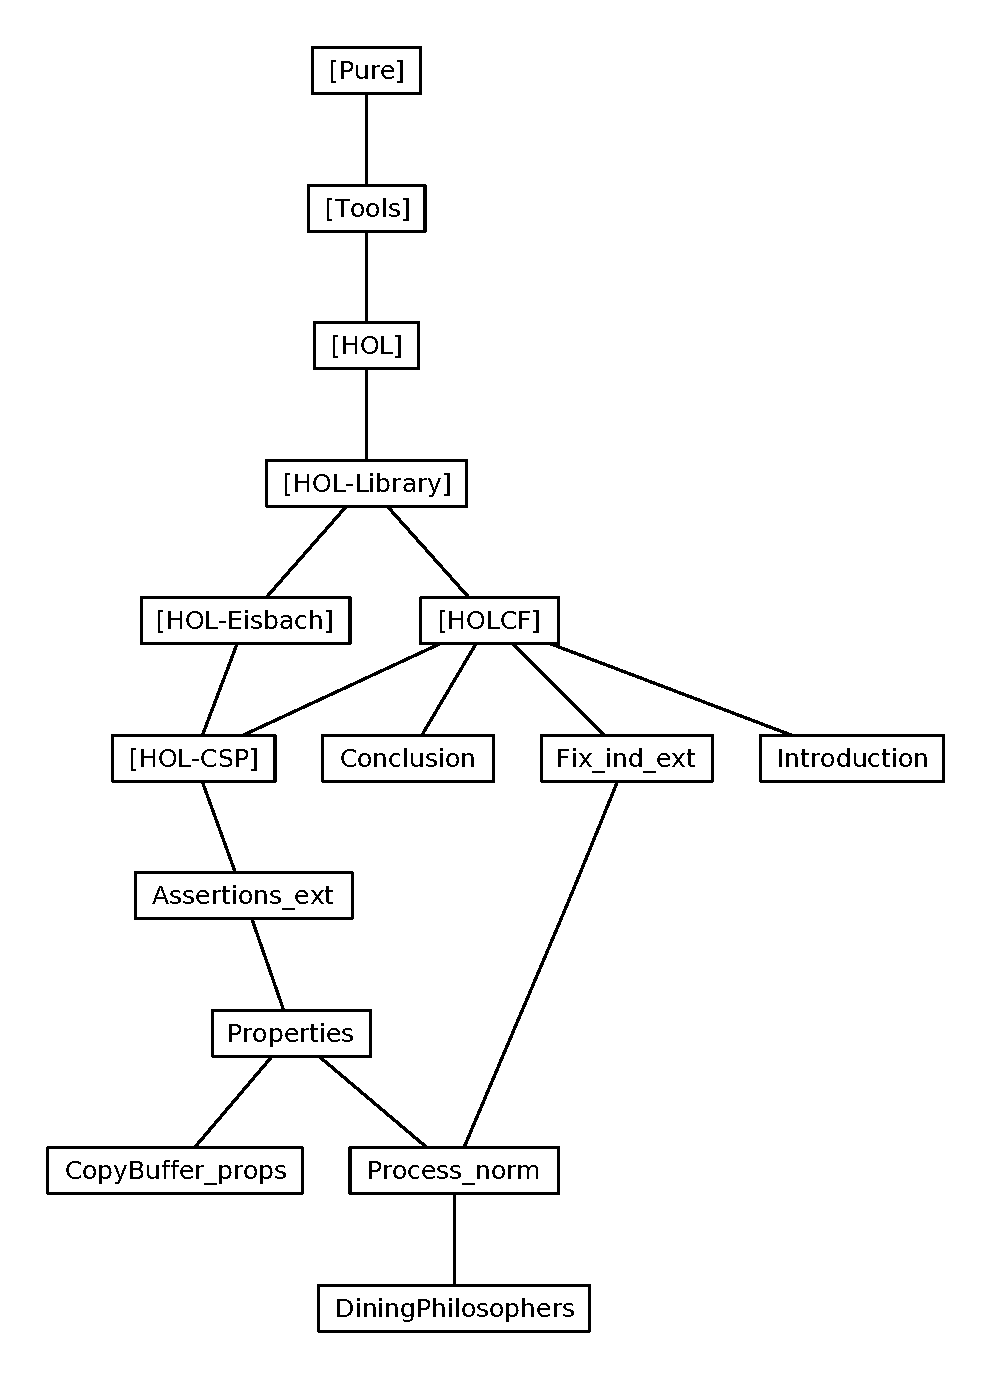
\includegraphics[width=.8\textwidth]{session_graph}
  \caption{The Dependency Graph of the Isabelle Theories.\label{fig:session-graph}}
\end{figure}

\clearpage

\chapter{Preliminaries}
\label{cha:perliminaries}
In this chapter, we introduce the technical preliminaries of our
formalization of the core DOM, namely a mechanism for hiding type
variables and the heap error monad.
\input{Hiding_Type_Variables}
\input{Heap_Error_Monad}

\chapter{References and Pointers}
\label{cha:pointers}
In this chapter, we introduce a generic type for object-oriented
references and typed pointers for each class type defined in the DOM
standard. 
\input{Ref}
\input{ObjectPointer}
\input{NodePointer}
\input{ElementPointer}
\input{CharacterDataPointer}
\input{DocumentPointer}
\input{ShadowRootPointer}

\chapter{Classes}
\label{cha:classes}
In this chapter, we introduce the classes of our DOM model. 
The definition of the class types follows closely the one of the
pointer types.  Instead of datatypes, we use records for our classes.
a generic type for object-oriented references and typed pointers for
each class type defined in the DOM standard.
\input{BaseClass}
\input{ObjectClass}
\input{NodeClass}
\input{ElementClass}
\input{CharacterDataClass}
\input{DocumentClass}

\chapter{Monadic Object Constructors and Accessors}
\label{cha:monads}
In this chapter, we introduce the moandic method definitions for the
classes of our DOM formalization. Again the overall structure follows
the same structure as for the class types and the pointer types.
\input{BaseMonad}
\input{ObjectMonad}
\input{NodeMonad}
\input{ElementMonad}
\input{CharacterDataMonad}
\input{DocumentMonad}

\chapter{The Core DOM}
\label{cha:dom}
In this chapter, we introduce the formalization of the core DOM, i.e.,
the most important algorithms for querying or modifying the DOM, as
defined in the standard. For more details, we refer the reader to
\cite{brucker.ea:core-dom:2018}.
\input{Core_DOM_Basic_Datatypes}
\input{Core_DOM_Functions}
\input{Core_DOM_Heap_WF}
\input{Core_DOM}

\chapter{Test Suite}
\label{cha:tests}
In this chapter, we present the formalized compliance test cases for
the core DOM. As our formalization is executable, we can
(symbolically) execute the test cases on top of our model. Executing
these test cases successfully shows that our model is compliant to the
official DOM standard. As future work, we plan to generate test cases
from our formal model (e.g.,
using~\cite{brucker.ea:interactive:2005,brucker.ea:theorem-prover:2012})
to improve the quality of the official compliance test suite. For more
details on the relation of test and proof in the context of web
standards, we refer the reader to
\cite{brucker.ea:standard-compliance-testing:2018}.
\input{Core_DOM_BaseTest} \input{Document_adoptNode}
\input{Document_getElementById} \input{Node_insertBefore}
\input{Node_removeChild} \input{Core_DOM_Tests}

{\small
  \bibliographystyle{abbrvnat}
  \bibliography{root}
}
\end{document}

%%% Local Variables:
%%% mode: latex
%%% TeX-master: t
%%% End:
